\section{The TensorFlow library}\label{sec:TensorFlow}

Google began development of TensorFlow in 2011, and it has since risen to preeminence as one of the two de facto libraries for deep learning in \lstinline{python}\footnote{The other is \lstinline{PyTorch}, which is developed by Facebook.} \cite{tensorflow}. The library implements tools for the development of a variety of deep-learning architectures, from fundamental linear algebra operations to interfaces with common layer types. At the core of the library is a computational graph structure constructed for numerical computations. This graph separates TensorFlow from other libraries for numerical \lstinline{python} applications. The graph does not execute an operation when it is defined but rather executes operations when asked to retrieve values for a specific variable in the graph. Writing code in TensorFlow is in this way similar to writing code in a traditional compiled language.

One of the challenges when writing scientific code in \lstinline{python} is that indexing and iteration in loops are notoriously slow by default, but they can be sped up considerably. Speeding up \lstinline{python} is achieved by avoiding \lstinline{python}'s built-in iterables and loop structures where possible. Instead we rely on interfaces to heavily optimized \lstinline{C}or \lstinline{C++} code. This is what allows us to perform quite demanding computations with TensorFlow.

\subsection{The computational graph}

To understand the program flow of the algorithms in subsequent sections we begin by introducing the fundamental concepts of TensorFlow code \footnote{The thesis code was written for the latest stable release of TensorFlow prior to the release of \lstinline{TF 2.0}. Accordingly, some modules may have moved, changed name or have been deprecated. Most notably in the versions prior to \lstinline{TF 2.0} eager execution was not the default configuration and as such the trappings of the implementation includes the handling of session objects.}. The heart of which is the computational graph. A graph defines all the operations needed for a model or another series of computations of interest. To retrieve values from the graph, we run it with an input, which is defined as a \lstinline{placeholder} tensor\footnote{We follow the TensorFlow nomenclature and define tensors as multidimensional arrays, unless otherwise explicitly stated.} object. TensorFlow \lstinline{placeholder} objects are special tensors that define the entry-point for the graph and acts as the input for a model, function or class. We include a code snippet with an associated graph in figure \ref{fig:graph}. It shows a simple program that computes a weight transformation of some input with a bias. The cost is included as the bracketed ellipses. When the forward pass is computed, or \textit{unrolled}, it becomes available for automatic differentiation. 

\begin{figure}
\centering
\begin{minipage}[c]{\linewidth}
\lstinputlisting[language=iPython]{../snippets/tf_graph.py}
\end{minipage}
\caption[A forward pass in TensorFlow]{This short script describes the setup required to compute a forward pass in a neural network as described in section \ref{sec:ANN}. Including more layers is as simple as a for loop and TensorFlow provides ample variations in both cell choices (RNN variations, convolutional cells etc.) and activation functions. This script is a modified version of figure 1 in \cite{tensorflow}}\label{fig:graph}
\end{figure}

\begin{figure}
\centering
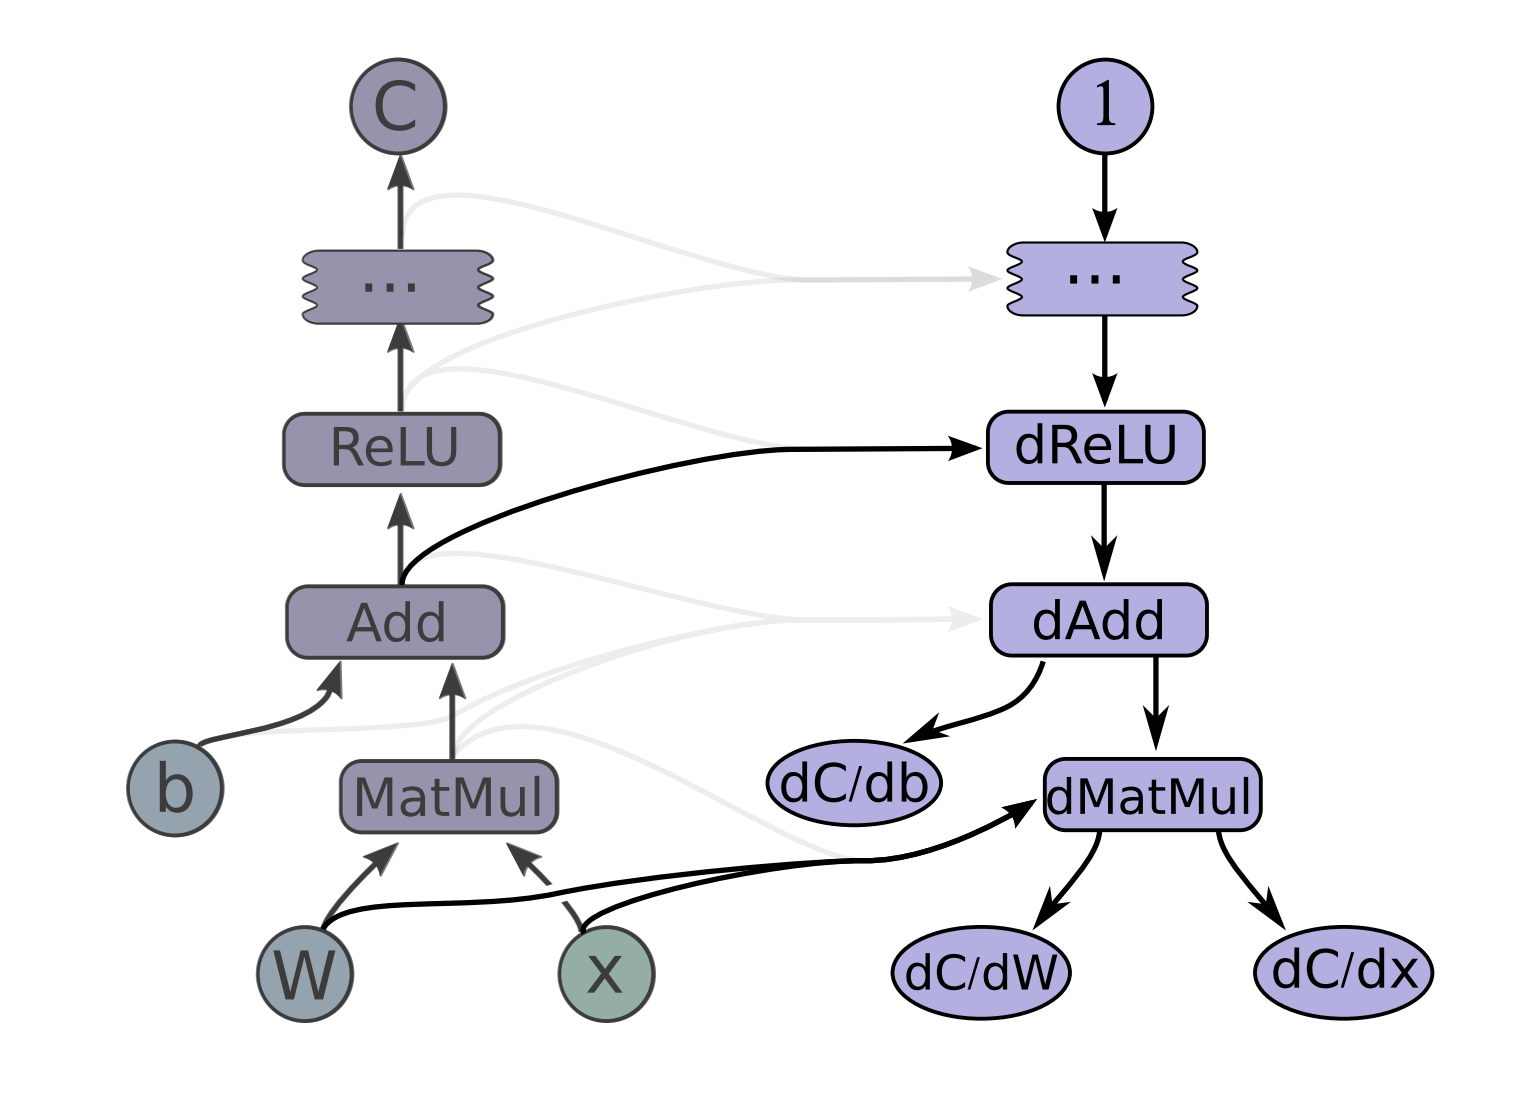
\includegraphics[height=6cm]{../snippets/gradients_graph.png}
\caption[Graph representation of the forward pass and gradients of a simple dense neural network]{A graph representation of the short script in figure \ref{fig:graph}, with respective gradients on the right. This figure is copied from \citet{tensorflow}}\label{fig:grad_graph}
\end{figure}

For the algorithms implemented in this thesis, we set up the computational graph to represent the forward pass, or predictive path, of the algorithm. The remainder then is then to compute the gradients required to perform gradient descent. TensorFlow provides direct access to find the gradients via \lstinline{tf.gradients(C, [I]k)} where \lstinline{[I]k} represents the set of tensors we wish to find the gradients of C with respect to. We use these gradients to perform the backpropagation algorithm, described in detail in section \ref{sec:ANN}. We show an illustration of the computational graph and the corresponding gradient nodes in figure \ref{fig:grad_graph}. The nodes in the figure represent TensorFlow operation types including variable declarations and operations on those including \lstinline{Add} and \lstinline{MatMul} operations.

To accommodate different gradient descent schemes, TensorFlow wraps the computation of gradients in optimizer modules. Defined in \lstinline{tf.train} these include stochastic gradient descent and ADAM, which we discuss in section \ref{sec:gd}. In this thesis, we will largely be using the ADAM optimizer.

We outline a basic TensorFlow script that goes through the basic steps outlined above. In the script we use the \lstinline{tf.train} module to compute the gradients needed to perform backpropagation of errors on the cost function assigned to the variable \lstinline{C}. Additionally we show the structure of a session and its run method to perform a backwards pass with respect to the loss \lstinline{C}:

\begin{minipage}{\linewidth}
\lstinputlisting[language=iPython]{../snippets/tf_script.py}
\end{minipage}